\documentclass[10pt]{beamer}
\usepackage{lmodern}
\usepackage[utf8]{vietnam}
\usepackage{amsmath}
\usefonttheme{structurebold}
\usetheme{Rochester}

\usepackage[backend=biber]{biblatex}

\addbibresource{presentation.bib}

\setbeamertemplate{navigation symbols}{\insertlogo}

\begin{document}
\author{Thu-Ngan Doan, Hoang-Quan Tran, Tan-Tho Huynh, Nhat-Dang Su, Diem-Uyen Phan-Dang}
\title{Efficiency of the Simplex Method}
\subtitle{Investigating on how fast Simplex Method will solve a problem in a given size.}
\logo{
\includegraphics[scale=.2]{img/fithcmuslogo.png}}
\institute{VNUHCM - University of Science}
\date{Spring 2022}
\subject{CSC10104 - Linear Programming}

\setbeamercovered{transparent}
\setbeamertemplate{navigation symbols}{}

\begin{frame}[plain]
\maketitle
\end{frame}

\begin{frame}
\frametitle{Mục lục}
\tableofcontents
\end{frame}

\section{Giới thiệu}
\begin{frame}{Giới thiệu}

\end{frame}

\section{Performance Measures}
\begin{frame}{Performance Measures}
Can be divied into two types:
\begin{itemize}
\item Worst case: asking how much efforts is needed to solve all problems of a given \textit{size}
\item Average case: looking at the average amount of effort, averaging over all problems of a giving \textit{size}. 
\end{itemize}
Worst-case analyses are generally easier than Average-case.
\end{frame}

\section{Measuring the Size of a Problem}
\begin{frame}{Measuring the Size of a Problem}

\end{frame}

\section{Measuring the Effort to Solve a Problem}
\begin{frame}{Measuring the Effort to Solve a Problem}

\end{frame}

\section{Worst-case Analysis of the Simplex Method}
\begin{frame}{Worst-case Analysis of the Simplex Method}
\begin{itemize}
\item Số phương án chấp nhận được tối đa có thể chọn là $\displaystyle \binom{n + m}{n}$.
\item Trong trường hợp xấu nhất, $n + m$ đạt giá trị lớn nhất khi $m = n$.
\item Ta có thể ước lượng một chặn trên và chặn dưới của $\displaystyle \binom{2n}{n}$\cite{Vanderbei2020}:
$$
\frac{2^{2n}}{2n} \leq \binom{2n}{n} \leq 2^{2n} \ (n \in \mathbb{N^+})
$$
\end{itemize}
\end{frame}
\begin{frame}{Worst-case Analysis of the Simplex Method (cont.) - Proof}
\begin{theorem}[Xấp xỉ Stirling\cite{weisstein}]
$$
\displaystyle
n! \operatorname*{\sim}_{n\to\infty} \sqrt{2\pi n}\left(\frac{n}{e}\right)^n
$$
\end{theorem}
Khai triển $\displaystyle \binom{2n}{n} = \frac{(2n)!}{(n!)^2}$\footnote{$\binom{n}{k} = \frac{n!}{(n - k)!k!}$}. Ta cũng có các xấp xỉ sau:
\begin{itemize}
\item $\displaystyle (2n)! \operatorname*{\sim}_{n\to\infty} 2\sqrt{\pi n} \left(\frac{2n}{e}\right)^{2n}$ 
\item $\displaystyle (n!)^2 \operatorname*{\sim}_{n\to\infty} 2\pi n \left(\frac{n}{e}\right)^{2n}$ 
\end{itemize}
Qua đó, $\displaystyle \binom{2n}{n} \operatorname*{\sim}_{n\to\infty} \frac{2\sqrt{\pi n} \left(\frac{2n}{e}\right)^{2n}}{2\pi n \left(\frac{n}{e}\right)^{2n}} =  \frac{2^{2n}}{\sqrt{\pi n}}$
\end{frame}

\begin{frame}{Worst-case Analysis of the Simplex Method (cont.) - Proof}
\begin{proof}
Gọi
$$
\displaystyle
L = \frac{\frac{2^{2n}}{2n}}{\frac{2^{2n}}{\sqrt{\pi n}}} = \frac{2^{2n}\sqrt{\pi n}}{2^{2n} 2n} = \frac{\sqrt{\pi}}{2\sqrt{n}} < 1,\ \forall n \in \mathbb{N^+}
$$
Do $L < 1$, ta có thể kết luận $\frac{2^{2n}}{2n} \leq \frac{2^{2n}}{\sqrt{\pi n}},\ \forall n \in \mathbb{N^+}
$. Khi đó
$$
\displaystyle
\frac{2^{2n}}{2n} \leq \frac{2^{2n}}{\sqrt{\pi n}} \leq 2^{2n} \iff \frac{2^{2n}}{2n} \leq \binom{2n}{n} \leq 2^{2n}
$$
\end{proof}
Trong trường hợp xấu nhất, thuật toán có độ phức tạp thuộc nhóm $\mathcal{O}(2^{2n})$. $2^{2n}$ \textbf{rất lớn} dù $n$ không lớn lắm. (e.g $n = 25$, $2^{50} = 1.1259\times 10^{15}$)
\end{frame}

\begin{frame}{Worst-case Analysis of the Simplex Method (cont.) - Example}
Năm 1972, V. Klee and G.J. Minty\cite{klee1970good} đề xuất bài toán Minty-Klee, theo đó phương pháp đơn hình cần ít nhất $2^n - 1$ lần lặp để giải:
\begin{equation*}
\sum_{j = 1}^{n} 2^{n - j} x_j \rightarrow \max
\end{equation*}
các ràng buộc
\begin{equation*}
\begin{aligned}
2\sum_{j = 1}^{i - 1} 2^{i - j}x_j + x_i &\leq 100^{i - 1} & (i = 1, 2, .., n)\\
x_j &\geq 0 & (j = 1, 2, .., n)
\end{aligned}
\end{equation*}
\end{frame}

\begin{frame}{Worst-case Analysis of the Simplex Method (cont.) - Example}
Xét 3 ràng buộc đầu tiên:
\begin{equation*}
\begin{aligned}
x_1 &\leq 1\\
4x_1 + x_2 &\leq 10^2\\
8x_1 + 4x_2 + x_3 &\leq 10^4
\end{aligned}
\end{equation*}
Dễ thấy đây chỉ là tập các cận trên của mỗi biến:
\begin{equation*}
\begin{aligned}
0 \leq x_1 &\leq 1\\
0 \leq x_2 &\leq 100\\
&\vdots\\
0 \leq x_n &\leq 100^{n - 1}
\end{aligned}
\end{equation*}
\end{frame}

\begin{frame}{Worst-case Analysis of the Simplex Method (cont.) - Example}
Đặt $\beta_i = 100^{i - 1}$. Với $n = 3$, bài toán được phát biểu như sau:
$$
4x_1 + 2x_2 + x_3 - 2\beta_1 - \beta_2 - \frac{1}{2}\beta_3 \rightarrow \max
$$
Các ràng buộc:
$$
\begin{aligned}
x_1 &\leq \beta_1\\
4x_1 + x_2 &\leq 2\beta_1 + \beta_2\\
8x_1 + 4x_2 + x_3 &\leq 4\beta_1 + 2\beta_2 + \beta_3
\end{aligned}
$$
\end{frame}

\begin{frame}{Worst-case Analysis of the Simplex Method (cont.) - Example}
Miền chấp thuận của bài toán Klee-Minty còn được gọi là Siêu lập phương\footnote{Siêu lập phương $n$ chiều có $2^n$ đỉnh.} Klee-Minty.
\begin{figure}
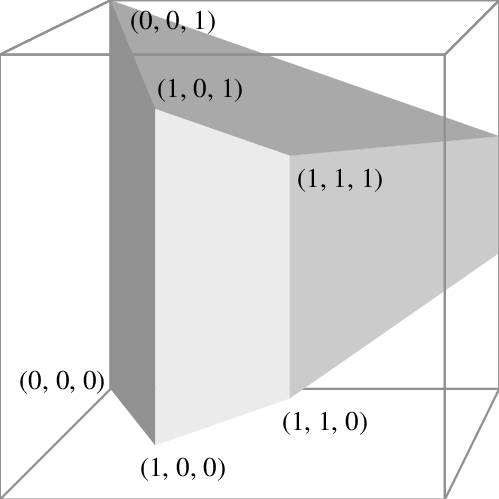
\includegraphics[scale=.15]{img/klee-minty-cube.png}
\caption{Ví dụ cho Siêu lập phương Klee-Minty với $n = 3$ và $\epsilon = \frac{1}{3}$}
\end{figure}
Phương pháp đơn hình sẽ xuất phát từ 1 đỉnh, đi qua tất cả các đỉnh trước khi tìm ra phương án tối ưu.
\end{frame}

\section{Empirical Average Performance of the Simplex Method}
\begin{frame}{Empirical Average Performance of the Simplex Method}

\end{frame}

\section{References}
\begin{frame}[allowframebreaks]{References}
\printbibliography
\end{frame}
\end{document}
